\documentclass[12pt]{article}
\usepackage{amsmath}
\usepackage{amssymb}
\usepackage{amsfonts}
\usepackage{polski}
\usepackage{verbatim}
\usepackage[utf8]{inputenc}
%\usepackage[polish]{babel}
\usepackage[T1]{fontenc}
\usepackage{graphicx}
%\usepackage[cp1250]{inputenc}
\usepackage{caption}
\usepackage{float}
\usepackage{enumitem}
\usepackage{hyperref}
\usepackage{url}
\usepackage[output-decimal-marker={,}]{siunitx}

\title{Prognozowanie sezonowe - porównanie metod \\
    \large Teoria Algorytmów i Obliczeń \\}
\author{Piotr Widomski}
\date{02.01.2022}

\begin{document}

\maketitle

\section{Cel projektu}

Celem projektu jest porównanie wydajności prognozowania sezonowych szeregów czasowych za pomocą maszyny \texttt{SARIMA} (\texttt{Seasonal ARIMA}) oraz liniowej kombinacji maszyn \texttt{ARIMA} działających na co $n$-tym elemencie szeregu.

\section{Użyte dane}

Do porównania metod użyte zostały dane przedstawiające średnią miesięczną temperaturę powietrza mierzoną na dublińskim lotnisku od roku 1941. Dane zostały pobrane z portalu inicjatywy \href{https://data.gov.ie/dataset/dublin-airport-monthly-data?package_type=dataset}{Open Data} prowadzonej przez rząd irlandzki. Pomiary wykonane zostały przez \href{https://www.met.ie/}{Met Éireann} - irlandzki narodowy serwis meteorologiczny i udostępnione na licencji CC Attribution 4.0.

Na potrzeby projektu użyty został wycinek danych zawierających pełne lata, od 1942 do 2019 roku, czyli 78 lat pomiarów. Dane te zostały podzielone na treningowe oraz testowe w stosunku około $80\%$, gdzie dane treningowe zawierają 62 lata, od 1942 do 2003 roku, a dane testowe - 15 lat, od 2004 do 2019 roku. Rok 2021 został pominięty ze względu na niekompletność danych, natomiast 2020 - z powodu brakujących danych z marca.

\section{Opis metod}

\subsection{ARIMA}

\texttt{ARIMA} jest klasą modelów, które opisują szereg na podstawie poprzednich wartości. Model \texttt{ARIMA} składa się z trzech procesów:

\begin{itemize}
    \item \texttt{AR} (autoregresyjny) - każda wartość jest liniową kombinacją pewnej liczby poprzednich wartości. Liczbę poprzednich wartości użytych przy obliczeniu następnej oznaczamy przez $p$, a a proces autoregresyjny z rzędem regresji $p$ - \texttt{AR(p)} i przedstawiamy następująco:
          \[
              y_t = \alpha + \phi_1y_{t-1} + \phi_2y_{t-2} + \dots + \phi_py_{t-p} + \epsilon_t
          \]
          gdzie $y_{t-i}$ jest $i$-tą poprzednią wartością ciągu w chwili $t$, $\phi_i$ jest współczynnikiem i-tej poprzedniej wartości, $\epsilon_t$ zaburzeniem w momencie t, a $\alpha$ - wartością podstawową.
    \item \texttt{MA} (średniej ruchomej) - każda wartość jest zależna od zaburzenia w chwili obecnej oraz wcześniejszych. Liczbę poprzednich zaburzeń uwzględnionych przy obliczeniu następnej wartości oznaczamy przez $q$, a proces średniej ruchomej rzędu $q$ - \texttt{MA(q)} i przedstawiamy:
          \[
              y_t = \alpha + \epsilon_t + \theta_1\epsilon_{t-1} + \theta_2\epsilon_{t-2} + \dots + \theta_q\epsilon_{t-q}
          \]
          gdzie $\epsilon_t$ jest zaburzeniem w momencie t, $\theta_i$ - współczynnikiem $i$-tego poprzedniego zaburzenia, a $\alpha$ - wartością podstawową.
    \item \texttt{I} (integracja) - w celu modelowania ciągów niestacjonarnych, model \texttt{ARIMA} może wykonywać różnicowanie pewnego stopnia, w celu operowania na bardziej stacjonarnym ciągu. W takim wypadku, zamiast następnej wartości, model prognozuje różnicę wartości. Jednak dzięki znajomości poprzedniej wartości możemy wyliczyć na podstawie różnicy następną wartość. Stopień różnicowania oznacza się przez $d$.
\end{itemize}

Łącząc powyższe procesy, otrzymujemy ogólny wzór modelu \texttt{ARIMA}:
\begin{gather*}
    y_t^* = \alpha + \sum^p_{i=1}\phi_iy^*_{t-i} + \sum^q_{i=1} + \theta_i\epsilon_{t-i} + \epsilon_t \\
    y_t^* = \Delta^dy_t
\end{gather*}
Poszczególne modele \texttt{ARIMA} definiuje się za pomocą trzech zmiennych całkowitych $p, d, q$ i zapisuje \texttt{ARIMA(p, d, q)}.

\subsection{SARIMA}

\texttt{SARIMA}, lub \texttt{Seasonal ARIMA}, jest rozszerzeniem modelu \texttt{ARIMA} wspierającym ciągi czasowe wykazujące sezonowość, czyli takie, które posiadają powtarzające się z pewną określaną częstością zmiany wartości. Częstość tę oznaczymy przez $S$.

Rozszerzenie to dodaje trzy nowe, analogiczne do modelu \texttt{ARIMA} procesy:
\begin{itemize}
    \item Sezonową autoregresję - stopień oznaczamy przez $P$
    \item Sezonową średnią ruchomą - stopień oznaczamy przez $Q$
    \item Sezonową integrację - stopień oznaczamy przez $D$
\end{itemize}
Procesy te łączą się z procesami modelu \texttt{ARIMA} w sposób multiplikatywny. Z tego powodu, w celu łatwiejszego zdefiniowania wzoru modelu \texttt{SARIMA}, zdefiniujmy operator poprzednika $B$:
\begin{gather*}
    By_t = y_{t-1} \\
    B^iy_t = y_{t-i}
\end{gather*}

Używając powyższego operatora możemy przekształcić model \texttt{ARIMA} do poniższej postaci:
\[
    \underbrace{\left(1 - \sum^p_{i=1} \phi_iB^i \right)}_\text{AR(p)}
    \cdot
    \underbrace{(1 - B)^d}_\text{I(d)}
    y_t =
    \underbrace{\left(1 + \sum^q_{i=1} \theta_iB^i \right)}_\text{MA{q}}
    \epsilon_t
\]

Uwzględniając procesy sezonowe, o postaci analogicznej do postaci procesów nie sezonowych, otrzymujemy ogólny wzór modelu \texttt{SARIMA}:
\begin{gather*}
    \underbrace{\left(1 - \sum^p_{i=1} \phi_iB^i \right)}_\text{AR(p)}
    \cdot
    \underbrace{\left(1 - \sum^P_{i=1} \Phi_iB^{Si} \right)}_\text{Sezonowe AR(P)}
    \cdot
    \underbrace{(1 - B)^d}_\text{I(d)}
    \cdot
    \underbrace{(1 - B^S)^D}_\text{Sezonowe I(d)}
    y_t = \\
    \underbrace{\left(1 + \sum^q_{i=1} \theta_iB^i \right)}_\text{MA{q}}
    \cdot
    \underbrace{\left(1 + \sum^Q_{i=1} \Theta_iB^{Si} \right)}_\text{Sezonowe MA{Q}}
    \epsilon_t
\end{gather*}

Poszczególne modele \texttt{SARIMA} definiuje się za pomocą zmiennych całkowitych niesezonowych $p, d, q$, zmiennych sezonowych $P, D, Q$ oraz częstości sezonowej $S$ i zapisuje \texttt{SARIMA(p, d, q) x (P, D, Q)S}.

\subsection{Kombinacja liniowa maszyn ARIMA}
\label{group-arima}

Model ten ma za zadanie prognozować kolejne elementy szeregu używając grup maszyn \texttt{ARIMA}. Każda z grup składa się z unikatowej liczby maszyn $n$, gdzie $n|S$ oraz $n > 1$. $i$-ta maszyna w grupie $n$ działa na co $n$-tym elemencie szeregu zaczynając od elementu $i$-tego. Dodatkowo w celu symulowania sezonowości maszyny te wykorzystują tylko ostatnie $S$ elementów szeregu. Oznacza to że taka maszyna ma postać \texttt{ARIMA($\frac{S}{n}$, 0, $\frac{S}{n}$)}.

Podsumowując, każda z maszyn w grupie prognozuje $i$-ty następny element szeregu wykorzystując co $i$-ty z ostatnich $S$ elementów szeregu. Łącząc wyniki maszyn w grupie otrzymujemy pełną prognozę.

Weźmy grupy maszyn spełniające powyższe warunki i ponumerujmy je $1, 2, \dots, n$. Oznaczmy przez $y_{i,t}$ element otrzymany z grupy $i$ w momencie $t$. Wartość tą możemy uzyskać stosując wzór modelu \texttt{ARIMA} z maszyną z grupy $i$, której indeks wewnątrz grupy jest równy $t \mod{i}$.
Stosując kombinację liniową maszyn \texttt{ARIMA} otrzymujemy następujący wzór na następny element:
\begin{gather*}
    y_t = \sum^n_{i=1}\alpha_iy_{i,t}
\end{gather*}
gdzie $\alpha_i$ jest współczynnikiem $i$-tej grupy. Model ten będzie również nazywany grupą maszyn \texttt{ARIMA} lub \texttt{ARIMA}.

\section{Implementacja}

\subsection{Biblioteka modeli}

Do budowy modeli została użyta biblioteka \href{https://www.statsmodels.org/stable/index.html}{\texttt{statsmodel}}, znajdująca się w pakiecie języka \texttt{Python} o tej samej nazwie, zapewniająca implementacje modeli \texttt{ARIMA} oraz rozszerzenia \texttt{SARIMA}. Dodatkowo biblioteka ta umożliwia automatyczne dobranie odpowiednich współczynników na podstawie danych wejściowych oraz parametrów modelu oraz udostępnia metody umożliwiające prognozowanie kolejnych elementów ciągu. Wykorzystane zostały również metody ułatwiające analizę używanego ciągu czasowego, takie jak rozkład sezonowy, ACF oraz PACF, które opisane zostały w następnym rozdziale.

Dodatkowo, w celu dobrania optymalnych parametrów modeli, użyta została biblioteka \href{https://alkaline-ml.com/pmdarima/}{\texttt{pmdarima}}, która umożliwia wyszukanie optymalnych parametrów modelu na podstawie ustalonych kryteriów, po czym zwraca maszynę utworzoną z dobranych przez siebie parametrów w implementacji kompatybilnej z tą, która znajduje się w bibliotece \texttt{statsmodels}.

\subsection{Metody analizy}

\subsubsection{Rozkład sezonowy}

Podczas analizy danych wykorzystany został rozkład sezonowy w modelu addytywnym. Rozkład ten polega na rozdzieleniu ciągu czasowego na trzy niezależne ciągi:
\begin{itemize}
    \item trend - określa tendencje zmian wartości ciągu w danym momencie.
    \item element sezonowy - określa wartość elementu, która wynika z sezonowości ciągu. Jeżeli ciąg wykazuje sezonowość, to element sezonowy jest cyklem.
    \item element losowy - pozostałość wartości elementu po odjęciu trendu oraz elementu sezonowego. Odpowiada zaburzeniu, które w modelu \texttt{ARIMA} oznaczamy symbolem $\epsilon$.
\end{itemize}
gdzie oryginalny ciąg możemy uzyskać poprzez ich sumę.

\subsubsection{Funkcja autokorelacji}

Funkcja autokorelacji (dalej ACF) opisuje w jakim stopniu element szeregu zależy od elementów poprzednich. Mając pomiary $y_1, y_2, \dots, y_n$ wykonane w równych odstępach czasu wartość funkcji autokorelacji dla opóźnienia $k$ zdefiniowana jest następująco:
\[
    r_k = \frac{\sum^{n-k}_{i=1}(y_i - \overline{y})(y_{i+k} - \overline{y})}
    {\sum^{n}_{i=1}(y_i - \overline{y})^2}
\]

Funkcji ta została użyta w celu dobrania odpowiednich parametrów modeli. Przy konstrukcji wykresów użyte zostały kolejne opóźnienia od $0$ do $30$.

\subsubsection{Funkcja częściowej autokorelacji}

Funkcja częściowej autokorelacji (dalej PACF) wyznacza częściową korelację szeregu czasowego z jego własnymi opóźnionymi wartościami. Mając pomiary $y_1, y_2, \dots, y_n$ wykonane w równych odstępach czasu wartość funkcji częściowej autokorelacji dla opóźnienia $k$ zdefiniowana jest następująco:
\begin{gather*}
    \rho_k = Corr(y_t, y_{t - k}) = \frac{\gamma_k}{\gamma_0} \\
    \gamma_k = Cov(y_t, y_{t - k})
\end{gather*}

Funkcji ta została użyta w celu dobrania odpowiednich parametrów modeli. Przy konstrukcji wykresów użyte zostały kolejne opóźnienia od $0$ do $30$.

\subsection{SARIMA}

Przed konstrukcją modelu wykonana została analiza danych za pomocą algorytmu \href{https://www.statsmodels.org/stable/generated/statsmodels.tsa.seasonal.seasonal_decompose.html}{rozkładu sezonowego} zaimplementowanego w bibliotece  udostępnionego przez bibliotekę \texttt{statsmodels}. Parametry modelu dobrane zostały zgodnie ze wskazówkami przedstawionymi przez Kotas Hatalis w \cite{A}.

Wynik rozkłądu prezentuje się następująco:

\begin{figure}[H]
    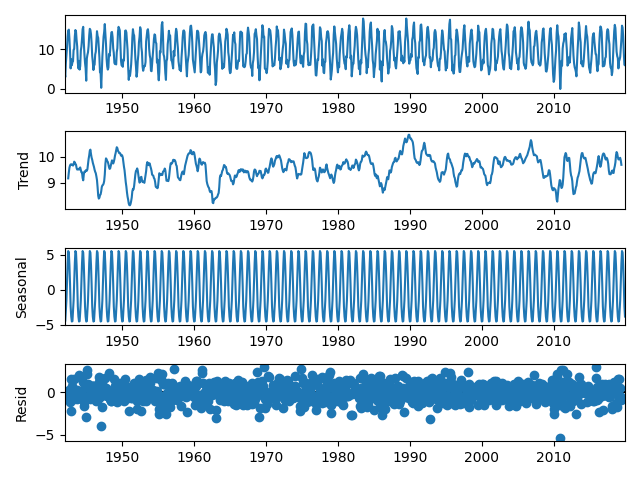
\includegraphics[width=\textwidth]{img/decomposition.png}
    \caption{Rozkład sezonowy średniej miesięcznej temperatury w latach od 1942 do 2019.
        Przestawia kolejno: wartość, trend, element sezonowy oraz element losowy.}
\end{figure}

Wykres przedstawia kolejno: wartość, trend, element sezonowy oraz element losowy każdego elementu ciągu. Z uwagi na dużą ilość elementów, wykres ten jest trudny w analizie. Z tego powodu, podczas analizy, skupiono się na pierwszych dziesięciu latach pomiarów:

\begin{figure}[H]
    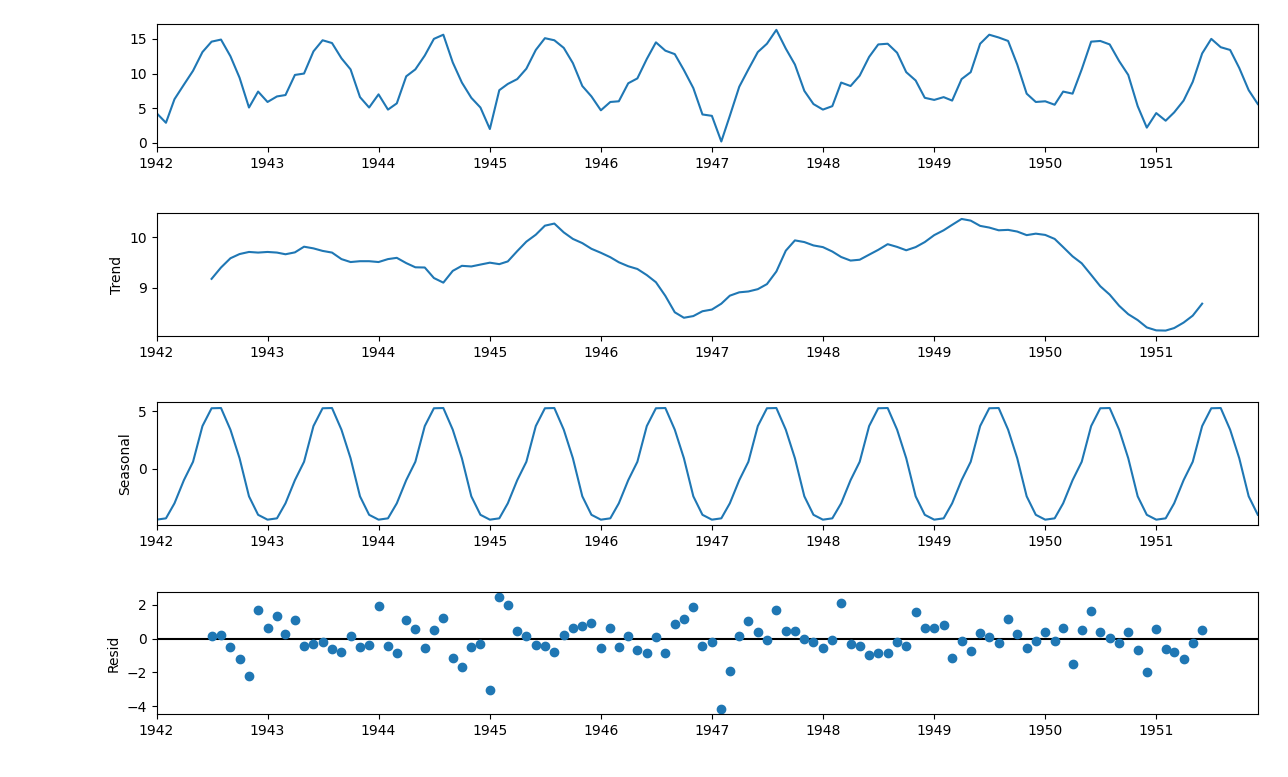
\includegraphics[width=\textwidth]{img/decomposition_10y.png}
    \caption{Rozkład sezonowy danych średniej miesięcznej temperatury w latach od 1942 do 1952.Przestawia kolejno: wartość, trend, element sezonowy oraz element losowy.}
\end{figure}

Z rozkładu danych zauważono, że zgodnie z oczekiwaniami dane posiadają stały element sezonowy o okresie wynoszącym dwanaście miesięcy. Element sezonowy jest stały, więc jako wartość parametru $D$ użyto $1$. Dodatkowo trend danych jest niejednoznaczny. Z tego powodu wartość parametru $d$ ustalono jako $0$.

Jako pomoc przy dobraniu pozostałych parametrów modelu \texttt{SARIMA} użyte zostały wykresy ACF oraz PACF:

\begin{figure}[H]
    \begin{minipage}{.5\textwidth}
        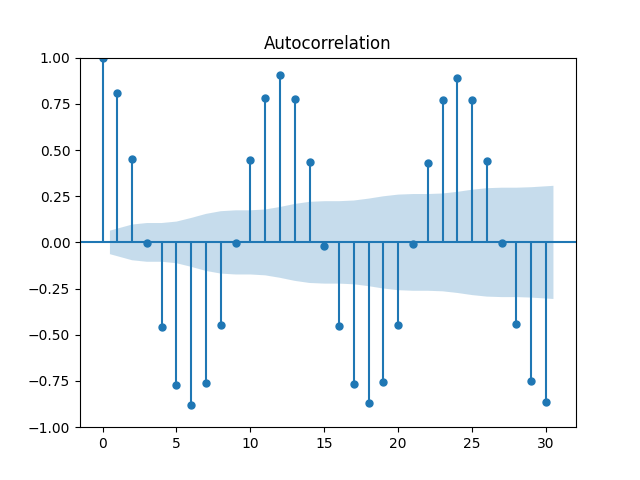
\includegraphics[width=\textwidth]{img/acf.png}
        \caption{Wykres autokorelacji}
    \end{minipage}
    \begin{minipage}{.5\textwidth}
        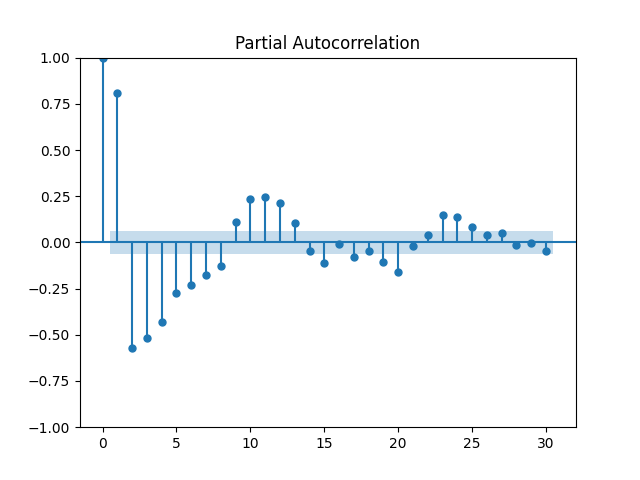
\includegraphics[width=\textwidth]{img/pacf.png}
        \caption{Wykres częsciowej autokorelacji}
    \end{minipage}
\end{figure}

Wykres ACF posiada największą wartość dla wartości $12, 24, \dots$, co potwierdza hipotezę o sezonowej częstości wynoszącej $12$ miesięcy. Wykres przyjmuje wartości ponad poziomem istotności dla dwóch pierwszych wartości (pomijając zerową), co powoduje że jako parametr $q$ użyta została wartość $2$. Dodatkowo wartość dla elementu $12$, czyli $S$, jest dodatnia. Z tego powodu parametr $P$ będzie przyjmował wartość dodatnią, a parametr $Q$ - wartość $0$.

Wykres PACF przyjmuje wartości ponad poziomem istotności dla pierwszej wartości (pomijając zerową), co sprawia że jako parametr $p$ użyta została wartość $1$.

Na podstawie analizy danych model \texttt{SARIMA(1, 0, 2) x (P, 1, 0)12}. Dokładna wartość $P$ została dobrana przy użyciu metody automatycznego dobierania parametrów modelu udostępnionej przez bibliotekę \texttt{pmdarima} i wyniosła $2$. Zatem ostateczna postać modelu wyniosła \texttt{SARIMA(1, 0, 2) x (2, 1, 0)12}.

\subsection{ARIMA}

Grupa maszyn \texttt{ARIMA} została zaimplementowana zgodnie z \hyperref[group-arima]{opisem}, z grupami o $n$ równym odpowiednio $2, 3, 4$ i $6$. Definicja grupy mówi, że maszyny działają na co $n$-tym elemencie z ostatnich $S$. Dlatego też każda maszyna ma postać \texttt{ARIMA($\frac{S}{n}$, 0, $\frac{S}{n}$)}, gdzie $d = 0$ wynika z analizy przeprowadzonej podczas konstrukcji maszyny \texttt{SARIMA}. Podczas stosowania kombinacji liniowej wyników, z powodu bliskich wartości przewidywanych przez każdą z grup, jako współczynnik dla każdej grupy przyjęto wartość $\frac{1}{4}$.

\section{Wyniki}

Na kolejnych wykresach szarym kolorem zaznaczona została pewność prognozy na poziomie $95\%$. Oznacza to prawdopodobieństwo $95\%$, że prawdziwa wartość będzie zawierać się w tym przedziale. Wyniki prezentują się następująco:

\begin{figure}[H]
    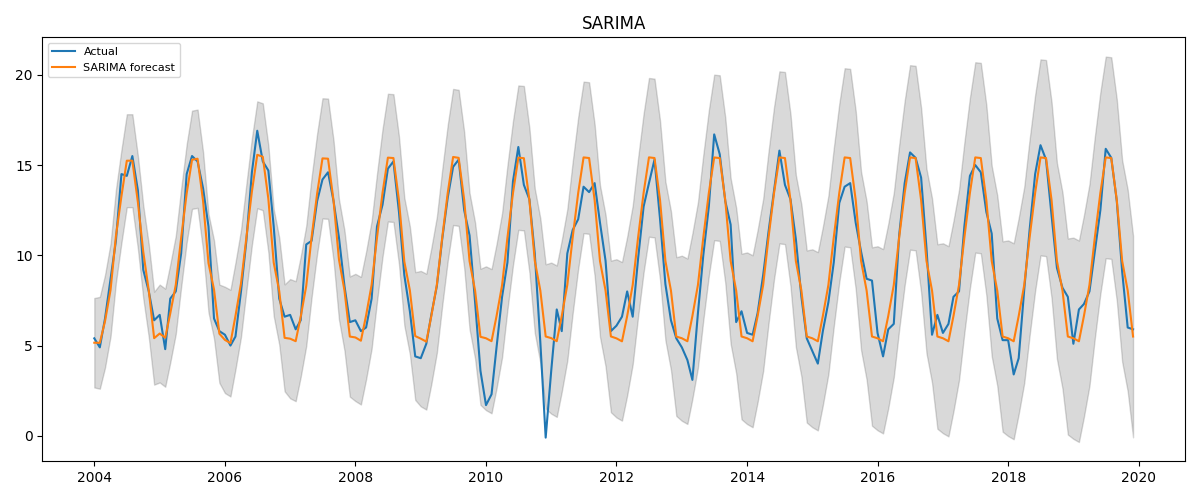
\includegraphics[width=\textwidth]{img/sarima.png}
    \caption{Wykres przewidywań modelu \texttt{SARIMA} z zaznaczoną pewnością $95\%$ oraz prawdziwych wartości}
\end{figure}

\begin{figure}[H]
    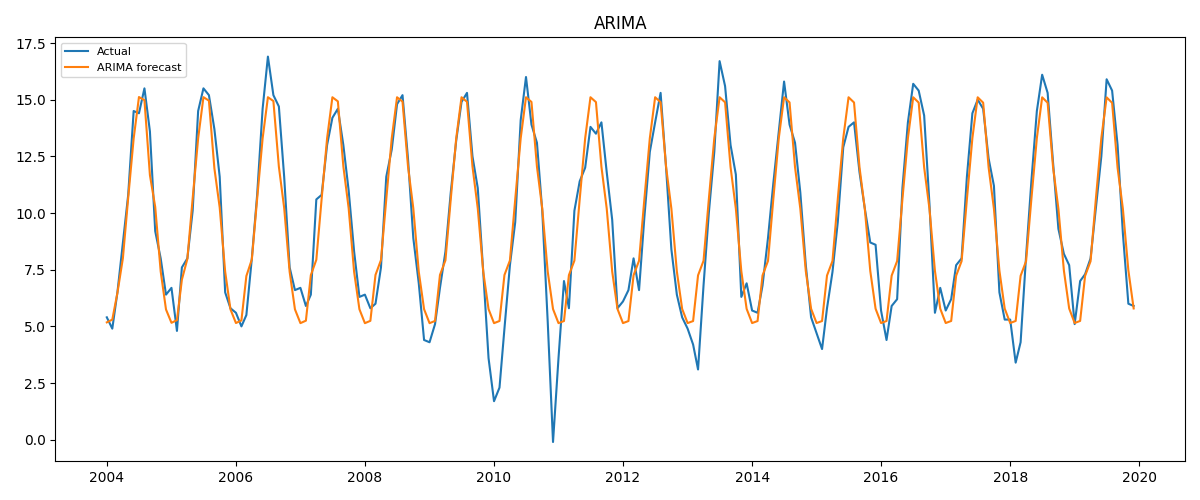
\includegraphics[width=\textwidth]{img/arima.png}
    \caption{Wykres przewidywań modelu kombinacji liniowej \texttt{ARIMA} oraz prawdziwych wartości}
\end{figure}

\begin{figure}[H]
    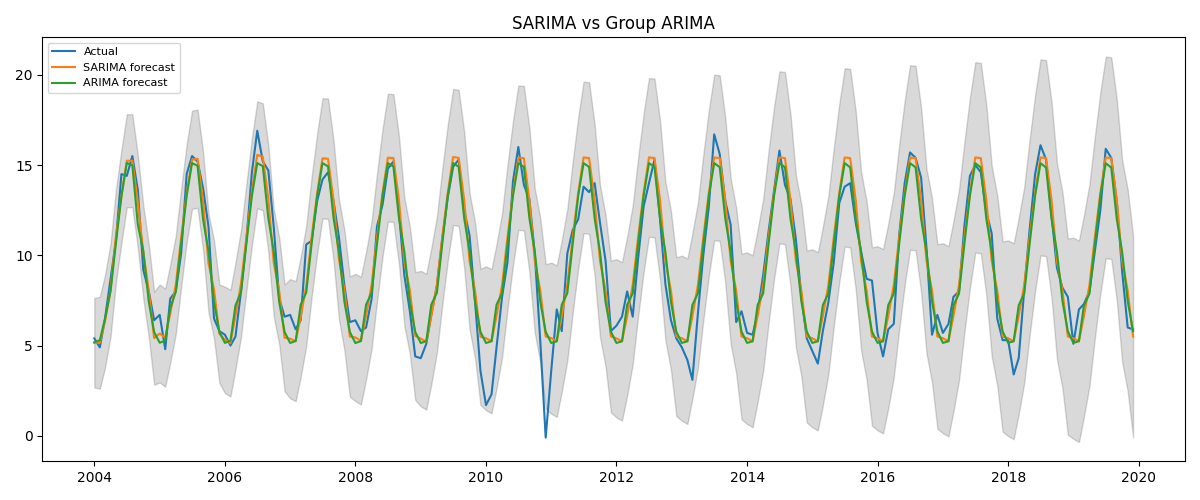
\includegraphics[width=\textwidth]{img/results.png}
    \caption{Wykres przewidywań obu modeli oraz prawdziwych wartości}
\end{figure}

\begin{figure}[H]
    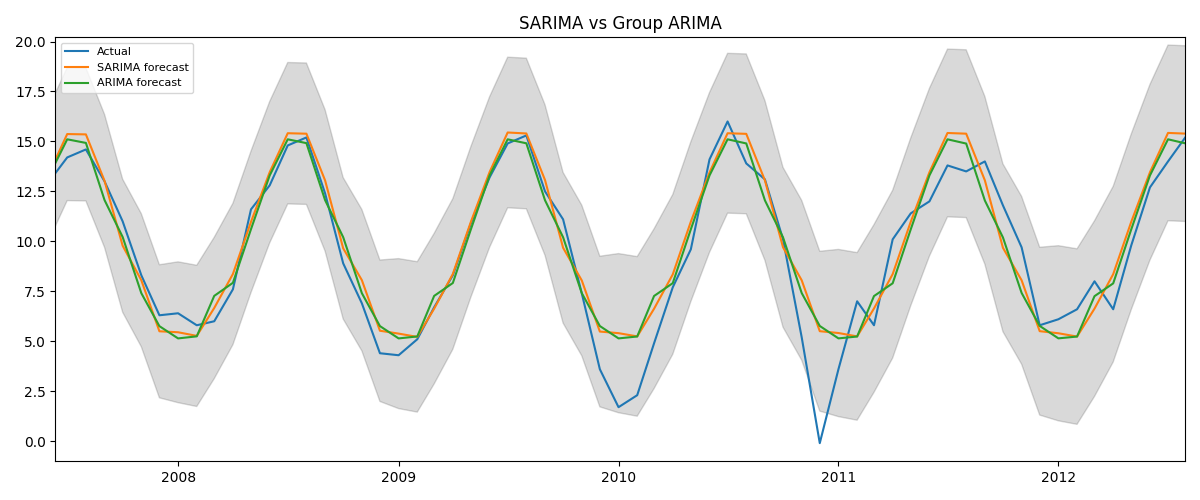
\includegraphics[width=\textwidth]{img/results_5y.png}
    \caption{Wykres przewidywań obu modeli oraz prawdziwych wartości przycięty do 5 lat}
\end{figure}

Model \texttt{SARIMA} osiągnął średni błąd kwadratowy równy $\num{1.2023}$ oraz średni błąd procentowy równy $\num{0.4212}$. Liniowa kombinacja maszyn \texttt{ARIMA} osiągnęła średni błąd kwadratowy równy $\num{1.2148}$ oraz średni błąd procentowy równy $\num{0.4346}$.

\newpage
\section{Wnioski}

Oba modele osiągnęły porównywalną efektywność oraz nie wykazują opóźnienia w zmianie trendu, co świadczy o świadomości sezonowej obu modeli. Jednocześnie wykresy obu modeli przypominają cykl, który nie wykazuje reakcji na nietypowe wartości, jak w przypadku przełomu 2009/2010 roku.

Przyglądając się wykresom można zauważyć, że model \texttt{SARIMA} posiada kształt bliższy wartościom rzeczywistym w okresie zimowym, kiedy wartości temperatury są najniższe i wachają się przez kilka miesięcy, przed ponownym wzrostem we wczesnej wiośnie. Natomiast model \texttt{ARIMA} lepiej przystosował się do wartości w okresie po nowym roku, gdzie często widzimy nagły skok, po którym następuje lekkie wygładzenie oraz ponowny wzrost.

Dobrane dane charakteryzują się niejednolitym trendem oraz niską względną różnicą wartości. Może to być jedna z przyczym obserwowanego zachowania danych.

\begin{thebibliography}{20}

    \bibitem[1]{A} K. Hatalis, \emph{Tutorial: Multistep Forecasting with Seasonal ARIMA in Python}, Data Science Central, 2018, \url{https://web.archive.org/web/20201205000439/https://www.datasciencecentral.com/profiles/blogs/tutorial-forecasting-with-seasonal-arima}.
\end{thebibliography}

\end{document}